\documentclass[a4paper,twoside,12pt]{article}
\usepackage[top=1.5cm,left=1.5cm,right=1.5cm,bottom=2cm]{geometry}

\usepackage[utf8]{inputenc}
\usepackage[T1]{fontenc}
\usepackage{lmodern}
\usepackage[brazilian]{babel}

\usepackage{graphicx}
\usepackage{subfig}
\usepackage{psfrag}
\usepackage{cite}
\usepackage[cmex10]{amsmath}
\usepackage{amssymb}
\usepackage{upgreek}
\usepackage{microtype}
\usepackage{titling}
\usepackage{courier}
\usepackage{url}
\usepackage{hyperref}
\hypersetup{
	colorlinks=true,
	linkcolor=blue,
	urlcolor=blue
}
\usepackage[makeroom]{cancel}

% Use the 'listings' package to add code and the 'color' package to generate the highlights
\usepackage{listings}
\usepackage{color}
\definecolor{grey}{rgb}{0.6,0.6,0.6}
\definecolor{codegreen}{rgb}{0,0.6,0}
\definecolor{codegray}{rgb}{0.5,0.5,0.5}
\definecolor{codepurple}{rgb}{0.58,0,0.82}
\definecolor{backcolour}{rgb}{0.95,0.95,0.92}
\lstset{language=Python,				% set it to Python language highlighting
	backgroundcolor=\color{backcolour},
	commentstyle=\color{codegreen},
	keywordstyle=\color{magenta},
	numberstyle=\tiny\color{codegray},
	stringstyle=\color{codepurple},
	basicstyle=\ttfamily\small,		% set size of fonts
	breaklines=true,				% set automatic line breaking
	linewidth=\textwidth,			% set size of code box
	showstringspaces=false}			% show spaces as underscores only inside strings

\title{\vspace{-2cm} Processamento Digital de Sinais e Aplicações em Acústica\\ Soluções para Tutorial 08 - Janelamento e \emph{Zero-Padding}}
\author{\url{https://github.com/fchirono/Aulas_PDS_Acustica}}

\begin{document}
	\date{}
	\maketitle

\setcounter{section}{2}

% ---------------------------------------------------------------------------------------------------------------
\subsection{DFT e \emph{Zero-Padding}}

\begin{enumerate}
	\setcounter{enumi}{1}
	\item A Figura \ref{fig:caso1_tempo} mostra os sinais discretos \texttt{x1} e \texttt{x2} em azul, com suas repetições periódicas em cinza. Nota-se que a junção entre os períodos é suave, com a última amostra de um período dando continuidade à primeira amostra do período seguinte de forma gradual.
	
	\item A Figura \ref{fig:caso1_freq} mostra os espectros de magnitude normalizados \texttt{|X1|/N1} e \texttt{|X2|/N2} em círculos azuis. Os intervalos de amostragem na frequência são $\Delta f_1 = f_s / N_1 = 1$ Hz e $\Delta f_2 = f_s / N_2 = 0.2$ Hz. Ambos os espectros possuem amostras de amplitude $A/2$ na frequência $f_0 = 1$ Hz do sinal original (e sua repetição espectral em $f = f_s - f_0 = 9$ Hz), e amostras de valor zero em todas as outras frequências; porém, o espectro \texttt{X2} possui mais amostras na frequência, devido ao maior número de pontos no sinal temporal discreto \texttt{x2}.
	
	\item A Figura \ref{fig:caso1_zp_tempo} mostra os sinais \texttt{x1} e \texttt{x2} com zero-padding no domínio do tempo; note que este sinal possui muito mais amostras de valor zero do que amostras do sinal original.
	
	A Figura \ref{fig:caso1_freq} mostra os espectros de magnitude com zero-padding em linhas vermelhas pontilhadas. Ambos os espectros com zero-padding possuem o mesmo intervalo de amostragem em frequência $\Delta f_{zp} = f_s / N_{zp} = 0.002$ Hz, resultando em dois espectros quase contínuos. Ao interpolar o espectro entre as amostras, observa-se que ambos os espectros possuem um lóbulo central em $f_0$ (e em sua repetição espectral $f_s-f_0$) e lóbulos laterais em frequências adjacentes, mas o espectro \texttt{X1} possui lóbulo central mais largo e lóbulos laterais mais altos do que \texttt{X2} devido ao menor número de pontos em \texttt{x1} -- o número inteiro de períodos no tempo faz com que as amostras em frequência coincidam com o pico da frequência fundamental e com os zeros do espectro ``contínuo''.
	
	Ao plotar o mesmo gráfico em decibéis, as amostras de magnitude zero tornam-se $-\infty$ dB e não aparecem na figura. 
\end{enumerate}


\begin{figure}[h!]
	\centering
	\subfloat[]{
		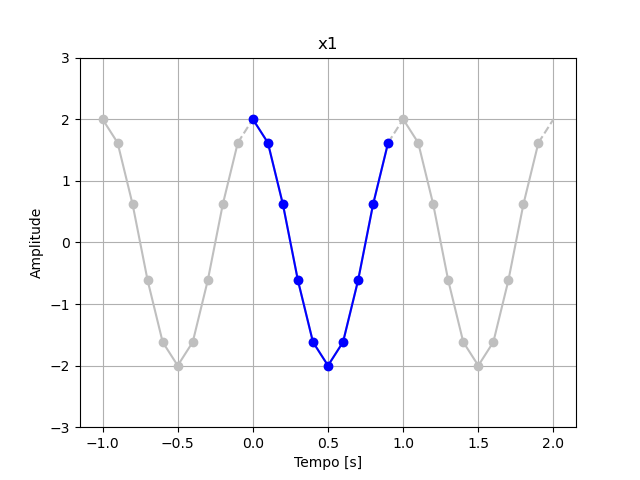
\includegraphics[width = 0.5\textwidth]{caso1_x1_tempo.png}
		\label{fig:caso1_x1_tempo}
	}
		\subfloat[]{
		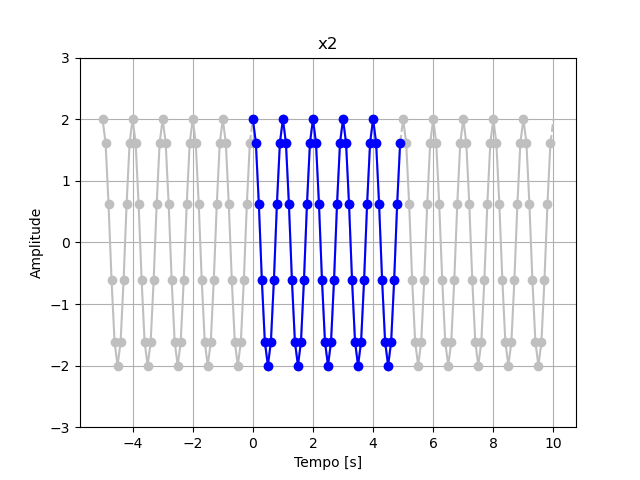
\includegraphics[width = 0.5\textwidth]{caso1_x2_tempo.png}
		\label{fig:caso1_x2_tempo}
	}
	\caption{Sinais \texttt{x1} \protect\subref{fig:caso1_x1_tempo} e \texttt{x2} \protect\subref{fig:caso1_x2_tempo} no domínio do tempo.}
	\label{fig:caso1_tempo}
\end{figure}


\begin{figure}[h!]
	\centering
	\subfloat[]{
		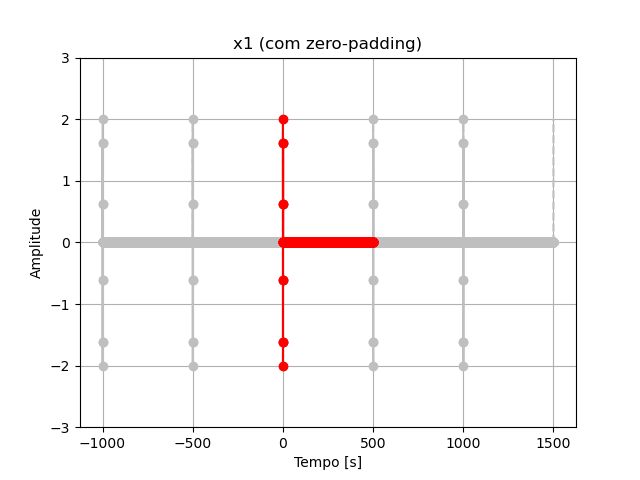
\includegraphics[width = 0.5\textwidth]{caso1_x1_zp_tempo.png}
		\label{fig:caso1_x1_zp_tempo}
	}
	\subfloat[]{
		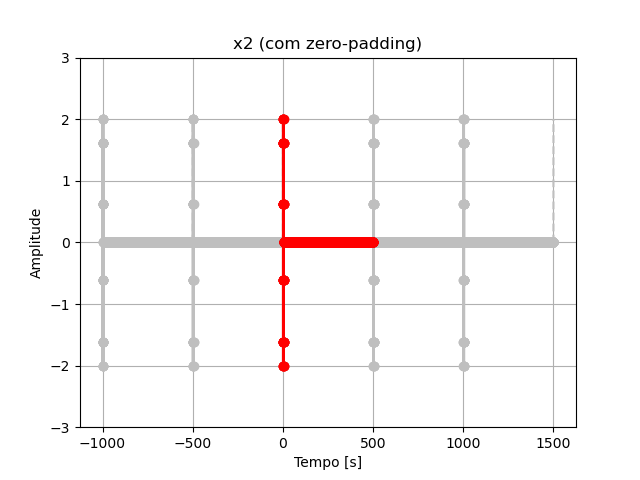
\includegraphics[width = 0.5\textwidth]{caso1_x2_zp_tempo.png}
		\label{fig:caso1_x2_zp_tempo}
	}
	\caption{Sinais \texttt{x1} \protect\subref{fig:caso1_x1_zp_tempo} e \texttt{x2} \protect\subref{fig:caso1_x2_zp_tempo} no domínio do tempo, com zero-padding.}
	\label{fig:caso1_zp_tempo}
\end{figure}

\begin{figure}[h!]
	\centering
	\subfloat[]{
		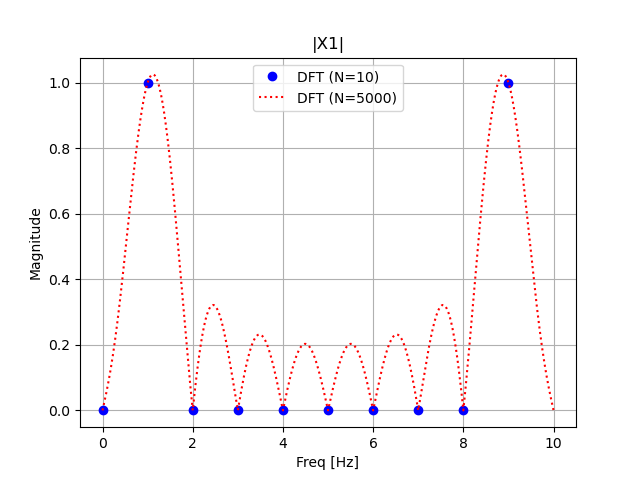
\includegraphics[width = 0.5\textwidth]{caso1_x1_freq.png}
		\label{fig:caso1_x1_freq}
	}
	\subfloat[]{
		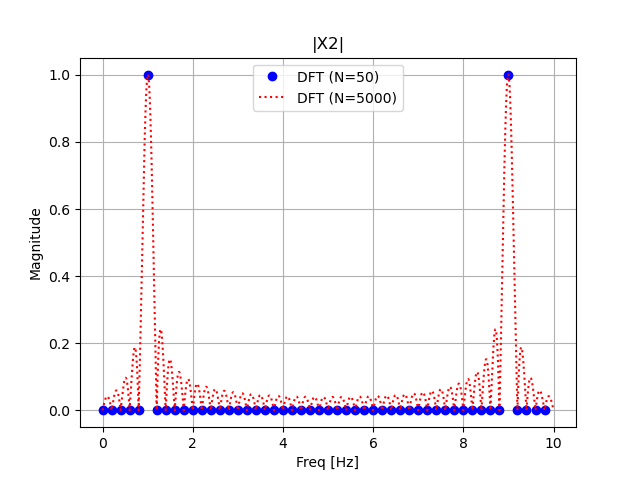
\includegraphics[width = 0.5\textwidth]{caso1_x2_freq.png}
		\label{fig:caso1_x2_freq}
	} \\
	\subfloat[]{
		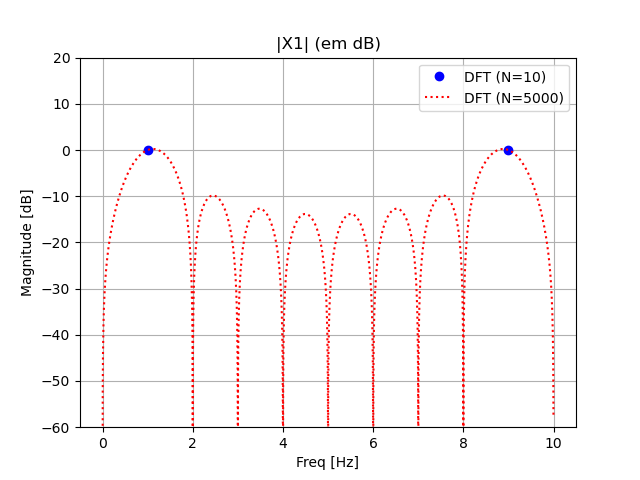
\includegraphics[width = 0.5\textwidth]{caso1_x1_freq_dB.png}
		\label{fig:caso1_x1_freq_dB}
	}
	\subfloat[]{
		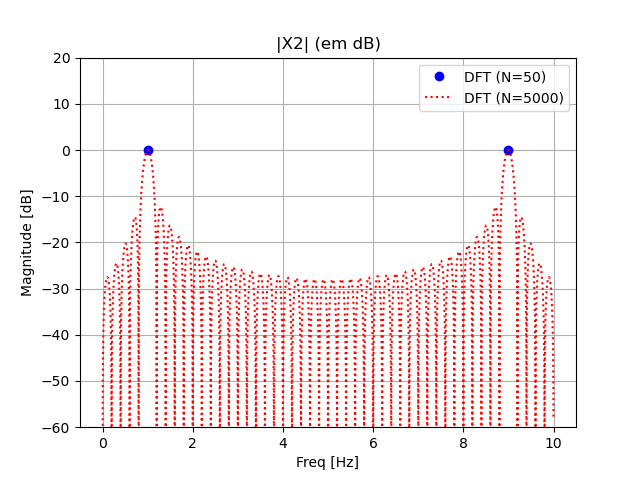
\includegraphics[width = 0.5\textwidth]{caso1_x2_freq_dB.png}
		\label{fig:caso1_x2_freq_dB}
	}
	\caption{Espectros em frequência  \texttt{|X1|/N1} \protect\subref{fig:caso1_x1_freq} e  \texttt{|X2|/N1} \protect\subref{fig:caso1_x2_freq} em escala linear, e \protect\subref{fig:caso1_x1_freq_dB}, \protect\subref{fig:caso1_x2_freq_dB} em escala logarítmica.}
	\label{fig:caso1_freq}
\end{figure}


% ---------------------------------------------------------------------------------------------------------------
\clearpage
\newpage
\subsection{Vazamento Espectral}

\begin{enumerate}
	\item A Figura \ref{fig:caso2_tempo} mostra os sinais discretos \texttt{x1} e \texttt{x2} em azul, com suas repetições periódicas em cinza. Nota-se que a junção entre os períodos (linha tracejada) agora é abrupta, com uma grande descontinuidade entre a última amostra de um período e a  primeira amostra do período seguinte.
	
	\item A Figura \ref{fig:caso2_freq} mostra os espectros de magnitude \texttt{|X1|/N1} e \texttt{|X2|/N2} sem zero-padding em círculos azuis, e com zero-padding em linhas vermelhas tracejadas. Desta vez, a frequência fundamental do sinal $f_0$ não coincide exatamente com nenhuma das amostras em frequência dos espectros \texttt{X1} ou \texttt{X2} (sem zero-padding), e portanto a magnitude do maior pico espectral não é uma forma robusta de estimar a amplitude do sinal senoidal original. Nota-se também que amostras em frequências $f \neq f_0$ apresentam magnitudes não-zero, apesar do sinal original não possuir componentes nestas frequências. Ambos os fenômenos são características de \emph{vazamento espectral}. 
	
	Os espectros com zero-padding são bastante similares ao caso anterior: novamente observa-se um lóbulo central de largura finita em torno de $f_0$ e diversos lóbulos laterais de magnitude decrescente em torno deste. Novamente, o espectro \texttt{X1} possui lóbulo central mais largo e lóbulos laterais mais altos do que \texttt{X2}, devido ao menor número de pontos no sinal original \texttt{x1} -- nota-se portanto que estes fatores fundamentais estão relacionados à duração do segmento de tempo discreto original, e não são afetados pelo presença (ou ausência) de zero-padding.
	
	Finalmente, observe que é mais fácil entender o vazamento espectral na DFT como \emph{uma condição específica de amostragem da DTFT}, ao invés de uma limitação ou ``defeito'' da DFT.
\end{enumerate}

\begin{figure}[h!]
	\centering
	\subfloat[]{
		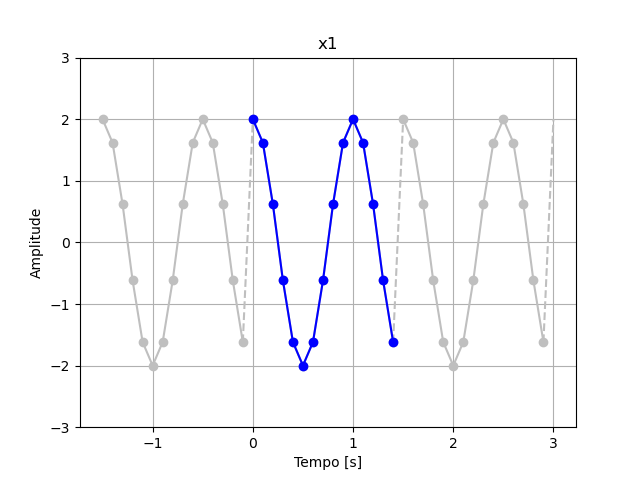
\includegraphics[width = 0.5\textwidth]{caso2_x1_tempo.png}
		\label{fig:caso2_x1_tempo}
	}
	\subfloat[]{
		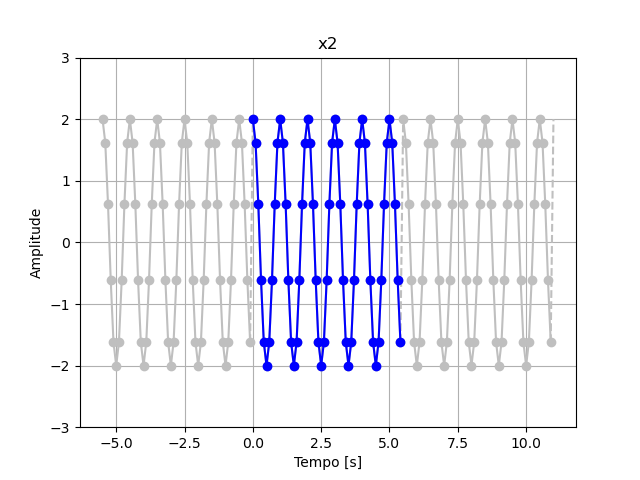
\includegraphics[width = 0.5\textwidth]{caso2_x2_tempo.png}
		\label{fig:caso2_x2_tempo}
	}
	\caption{Sinais \texttt{x1} \protect\subref{fig:caso1_x1_tempo} e \texttt{x2} \protect\subref{fig:caso1_x2_tempo} no domínio do tempo.}
	\label{fig:caso2_tempo}
\end{figure}


\begin{figure}[h!]
	\centering
	\subfloat[]{
		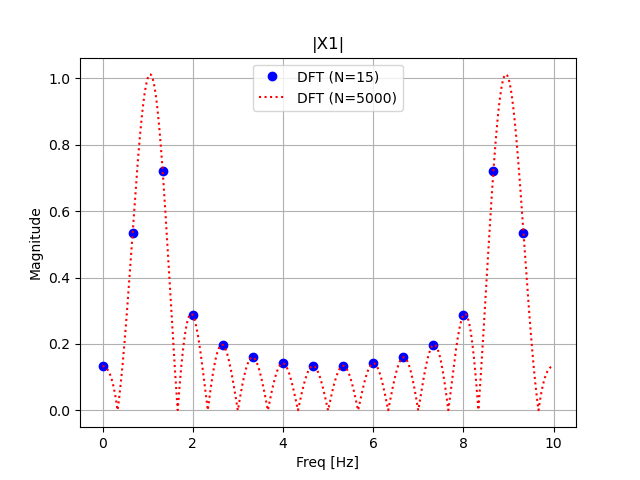
\includegraphics[width = 0.5\textwidth]{caso2_x1_freq.png}
		\label{fig:caso2_x1_freq}
	}
	\subfloat[]{
		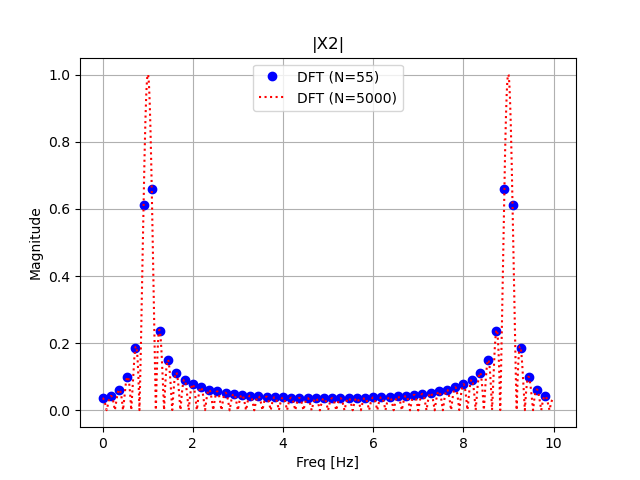
\includegraphics[width = 0.5\textwidth]{caso2_x2_freq.png}
		\label{fig:caso2_x2_freq}
	}\\
	\subfloat[]{
	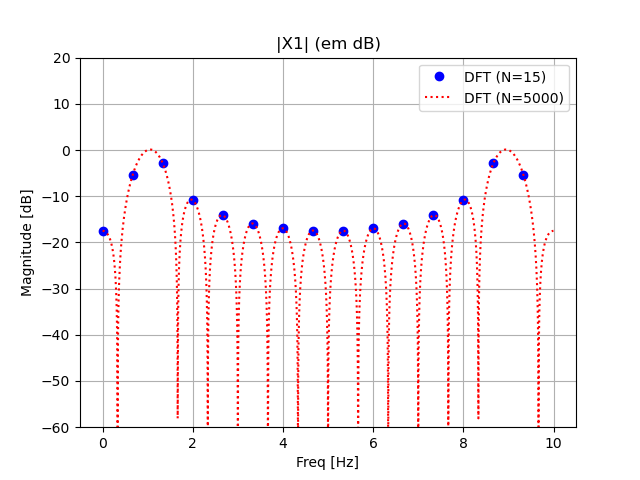
\includegraphics[width = 0.5\textwidth]{caso2_x1_freq_dB.png}
	\label{fig:caso2_x1_freq_dB}
	}
	\subfloat[]{
	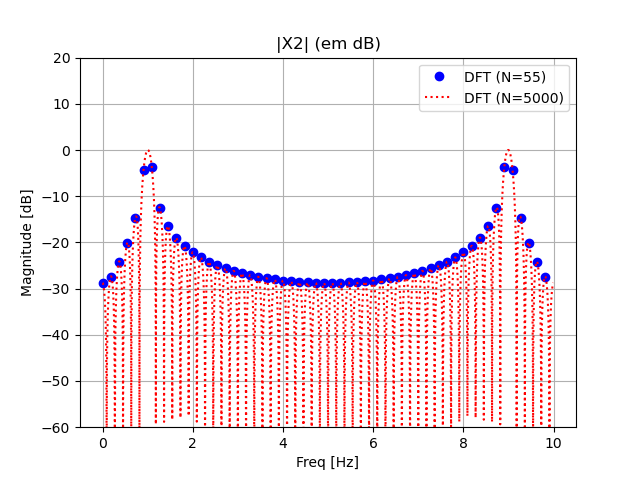
\includegraphics[width = 0.5\textwidth]{caso2_x2_freq_dB.png}
	\label{fig:caso2_x2_freq_dB}
	}
	\caption{Espectros em frequência \texttt{X1} \protect\subref{fig:caso2_x1_freq} e \texttt{X2} \protect\subref{fig:caso2_x2_freq} em escala linear, e \protect\subref{fig:caso2_x2_freq_dB}, \protect\subref{fig:caso2_x2_freq_dB} em escala logarítmica.}
	\label{fig:caso2_freq}
\end{figure}


% ---------------------------------------------------------------------------------------------------------------
\clearpage
\newpage
\subsection{Resolução Espectral}

\begin{enumerate}
	\item A Figura \ref{fig:caso3_tempo} mostra os sinais discretos \texttt{x1} e \texttt{x2}. Devido à baixa amplitude da segunda componente em frequência, não é possível identificar a sua presença a partir da visualização do sinal temporal discreto. 
	
	\item A Figura \ref{fig:caso3_freq} mostra os espectros normalizados com e sem zero-padding. Espera-se observar dois picos nas frequências $f_0 = 1$ Hz e $f_{0b} \approx 2.83$ Hz, com amplitudes $A/2 = 1$ e $A_b/2 = 0.05$. Novamente pode-se observar os efeitos de vazamento espectral em ambos os casos: o espectro de \text{x1} (de duração $T_1$) mascara o pico em $f_{0b}$, dado que seus lóbulos laterais possuem magnitude maior que $0.05$ em torno de $2.83$ Hz. O espectro de \texttt{x2} (de duração $T_2$) permite identificar um pico em $2.83$ Hz, devido aos seus lóbulos laterais de magnitude reduzida. A magnitude deste pico é uma combinação da amplitude $A_b/2$ do sinal de $2.83$ Hz com a contribuição de vazamento espectral da componente de $1$ Hz.
\end{enumerate}

\begin{figure}[h!]
	\centering
	\subfloat[]{
		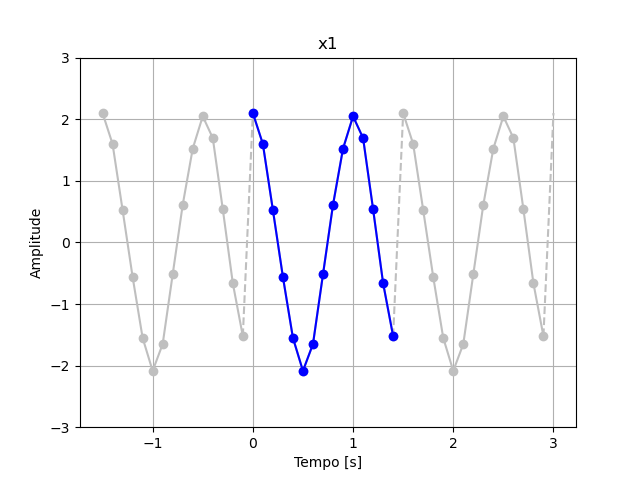
\includegraphics[width = 0.5\textwidth]{caso3_x1_tempo.png}
		\label{fig:caso3_x1_tempo}
	}
	\subfloat[]{
		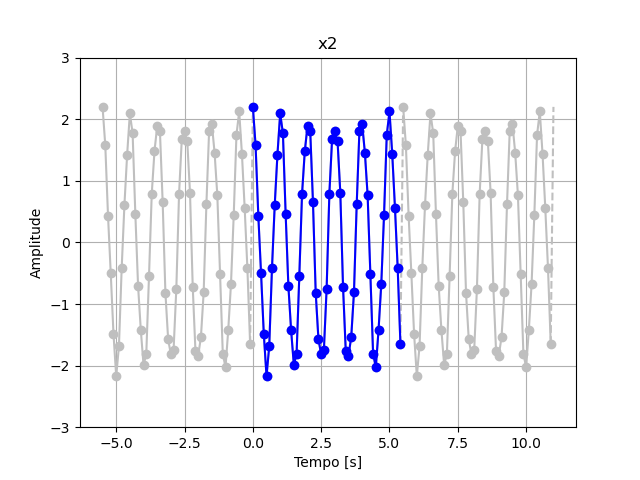
\includegraphics[width = 0.5\textwidth]{caso3_x2_tempo.png}
		\label{fig:caso3_x2_tempo}
	}
	\caption{Sinais \texttt{x1} \protect\subref{fig:caso1_x1_tempo} e \texttt{x2} \protect\subref{fig:caso1_x2_tempo} no domínio do tempo.}
	\label{fig:caso3_tempo}
\end{figure}


\begin{figure}[h!]
	\centering
	\subfloat[]{
		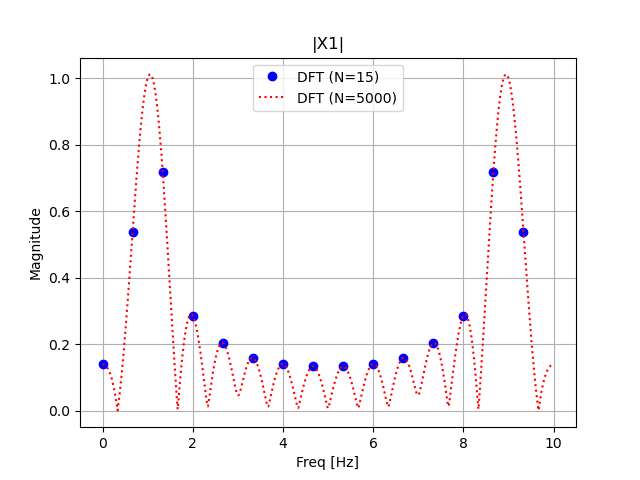
\includegraphics[width = 0.5\textwidth]{caso3_x1_freq.png}
		\label{fig:caso3_x1_freq}
	}
	\subfloat[]{
		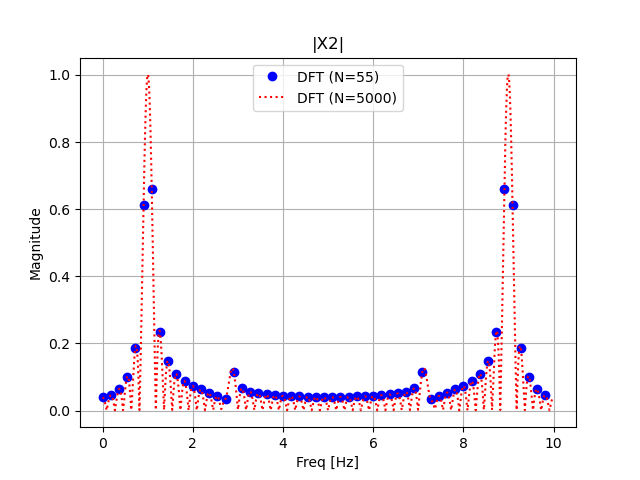
\includegraphics[width = 0.5\textwidth]{caso3_x2_freq.png}
		\label{fig:caso3_x2_freq}
	} \\
	\subfloat[]{
	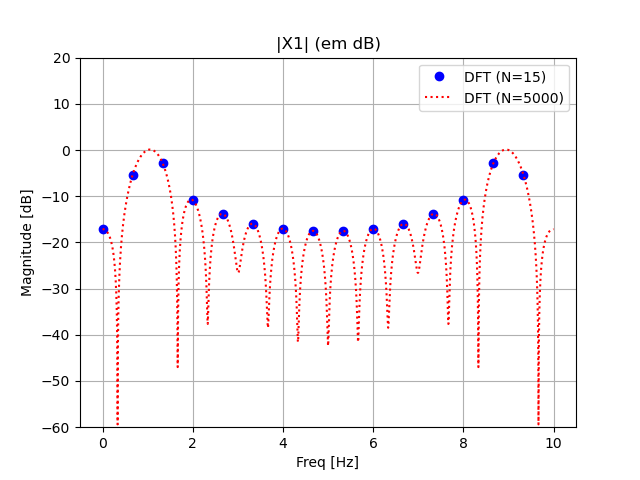
\includegraphics[width = 0.5\textwidth]{caso3_x1_freq_dB.png}
	\label{fig:caso3_x1_freq_dB}
	}
	\subfloat[]{
	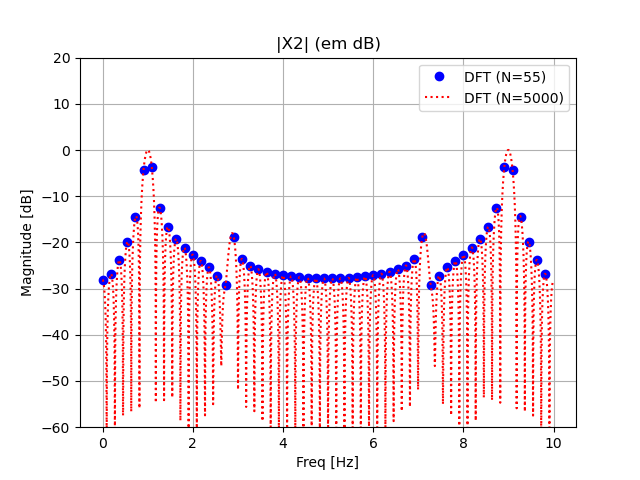
\includegraphics[width = 0.5\textwidth]{caso3_x2_freq_dB.png}
	\label{fig:caso3_x2_freq_dB}
	}
	\caption{Espectros em frequência \texttt{X1} \protect\subref{fig:caso3_x1_freq} e \texttt{X2} \protect\subref{fig:caso3_x2_freq} em escala linear, e \protect\subref{fig:caso3_x2_freq_dB}, \protect\subref{fig:caso3_x2_freq_dB} em escala logarítmica.}
	\label{fig:caso3_freq}
\end{figure}

% ---------------------------------------------------------------------------------------------------------------
\clearpage
\newpage
\subsection{Janelamento}

\begin{enumerate}
	\item A Figura \ref{fig:caso4_tempo} mostra os sinais discretos \texttt{x1} e \texttt{x2} com janelamento. Nota-se que a função de janelamento Hann reduz o início e o fim do segmento original para aproximadamente zero, forçando uma junção suave entre as repetições periódicas.
	
	\item A Figura \ref{fig:caso4_freq} mostra os espectros normalizados com janela Hanning, com e sem zero-padding. Em comparação com a Figura \ref{fig:caso3_freq} (janela retangular), nota-se que o espectro com janela Hann possui um lóbulo central mais largo e lóbulos laterais mais baixos. Neste exemplo, a redução nos lóbulos laterais permite observar claramente a componente em frequência de menor amplitude no caso \texttt{X2}, enquanto no caso \texttt{X1} a sua presença pode ser notada mas não é muito clara.
	
	\item Os picos espectrais apresentam magnitudes menores ao usar a função de janelamento Hann. Considere que a função de janelamento tipicamente possui valores menores que 1, e portanto o sinal ``janelado'' terá menos energia que o sinal original. É possível normalizar o espectro pelo coeficiente $\sum w[n]/N$ para corrigir este efeito, caso desejado.
	
	\item A janela Hann apresenta lóbulos laterais mais baixos que a janela retangular, e portanto permite a identificação de componentes em frequências distintas e com baixas amplitudes, como demonstrado neste exercício. Porém, a janela Hann também apresenta lóbulo lateral mais largo que a janela retangular, e não permite a resolução de componentes em frequências próximas e amplitudes similares; neste caso, a janela retangular é uma opção mais apropriada.
\end{enumerate}


\begin{figure}[h!]
	\centering
	\subfloat[]{
		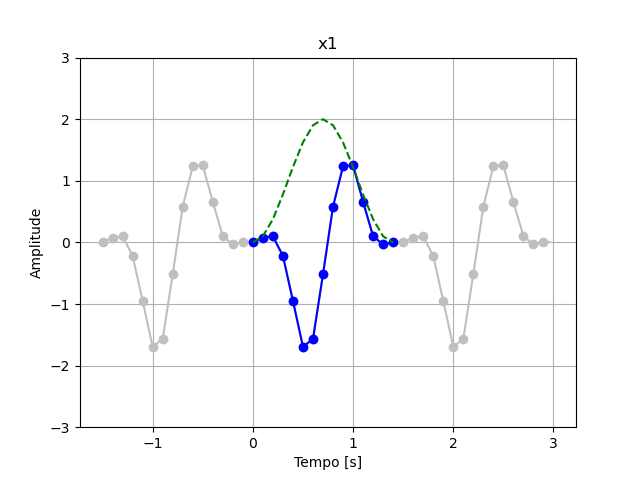
\includegraphics[width = 0.5\textwidth]{caso4_x1_tempo.png}
		\label{fig:caso4_x1_tempo}
	}
	\subfloat[]{
		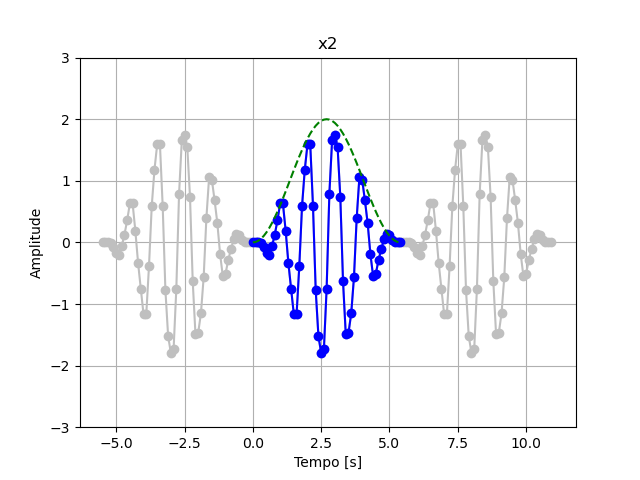
\includegraphics[width = 0.5\textwidth]{caso4_x2_tempo.png}
		\label{fig:caso4_x2_tempo}
	}
	\caption{Sinais \texttt{x1} \protect\subref{fig:caso4_x1_tempo} e \texttt{x2} \protect\subref{fig:caso4_x2_tempo} no domínio do tempo.}
	\label{fig:caso4_tempo}
\end{figure}


\begin{figure}[h!]
	\centering
	\subfloat[]{
		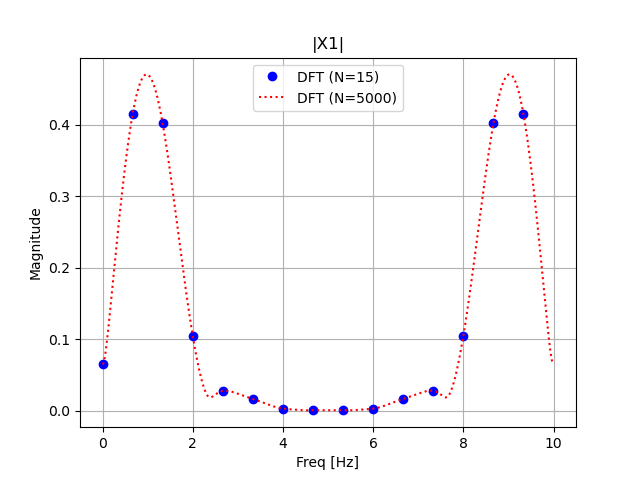
\includegraphics[width = 0.5\textwidth]{caso4_x1_freq.png}
		\label{fig:caso4_x1_freq}
	}
	\subfloat[]{
		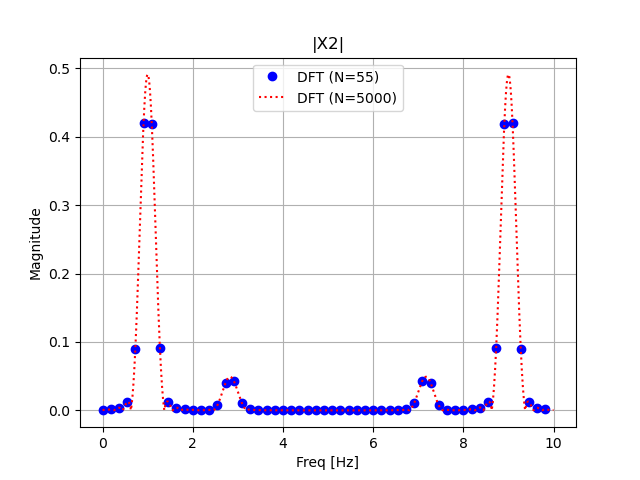
\includegraphics[width = 0.5\textwidth]{caso4_x2_freq.png}
		\label{fig:caso4_x2_freq}
	} \\
	\subfloat[]{
		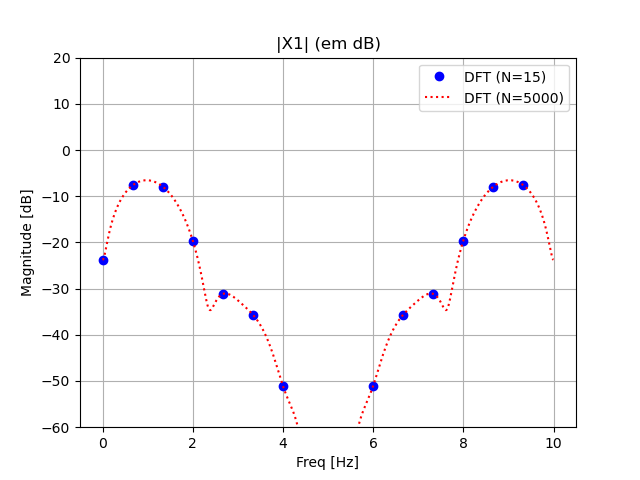
\includegraphics[width = 0.5\textwidth]{caso4_x1_freq_dB.png}
		\label{fig:caso4_x1_freq_dB}
	}
	\subfloat[]{
		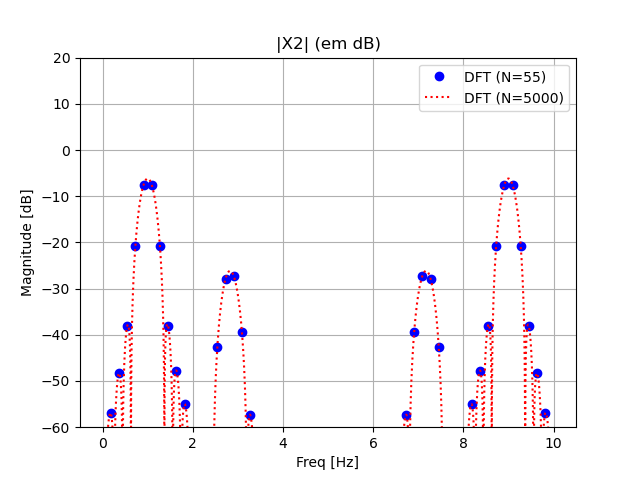
\includegraphics[width = 0.5\textwidth]{caso4_x2_freq_dB.png}
		\label{fig:caso4_x2_freq_dB}
	}
	\caption{Espectros em frequência \texttt{X1} \protect\subref{fig:caso4_x1_freq} e \texttt{X2} \protect\subref{fig:caso4_x2_freq} em escala linear, e \protect\subref{fig:caso4_x2_freq_dB}, \protect\subref{fig:caso4_x2_freq_dB} em escala logarítmica.}
	\label{fig:caso4_freq}
\end{figure}

\end{document}
